The \Kieker{} download site\footnote{\KiekerDownloadURL{}} includes an additional %
example \file{\JavaEEServletExampleName}. Using the sample Java Web application %
iBATIS JPetStore\footnote{\url{http://ibatis.apache.org/}}, this example %
demonstrates how to employ \KiekerMonitoringPart{} for monitoring a Java application %
running in a Java~EE container---in this case, Apache Tomcat\footnote{\url{http://tomcat.apache.org/}}. %
Monitoring probes based on the Java~EE Servlet API %
and AspectJ are used to monitor execution, trace, and session data (see Section~\ref{chap:aspectJ}).

\section{Preparation of the Tomcat Servlet Container}

\TODO{update}

\begin{compactenum}
\item Copy the files \file{\mainJar} and \file{\aspectJWeaverJar} from %
\Kieker{}'s binary distribution to the Tomcat's \dir{lib/} directory.
\item Copy the file \file{\servletWar} from \Kieker{}'s %
binary distribution to the Tomcat's \dir{webapps/} directory.
\item Tomcat's \dir{lib/} directory contains the files \file{kieker.monitoring.properties} %
and \file{aop.xml} --- the configuration of \KiekerMonitoringPart{} and the %
AspectJ-based instrumentation. %
\item
 Tomcat's start script \file{bin/catalina.\{sh|bat\}} file was modified to add the location %
of the \file{kieker.\-moni\-toring.properties} and the AspectJ agent to the argument %
list of the JVM call:
\end{compactenum}

\enlargethispage{1cm}

% \setPropertiesListing
% \lstinputlisting[firstline=188,firstnumber=188,lastline=190,caption={Excerpt from catalina.sh (for \UnixLikeSystems)},numbers=left]{\JavaEEServletExampleDir/Tomcat6.0.18WithJpetStore-withInstrumentedJPetStore/bin/catalina.sh}
% 
% \setPropertiesListing
% \lstinputlisting[firstline=121,firstnumber=121,lastline=123,caption={Excerpt from catalina.bat (for Windows)},numbers=left]{\JavaEEServletExampleDir/Tomcat6.0.18WithJpetStore-withInstrumentedJPetStore/bin/catalina.bat}

%% BEGIN: Windoof
% set JAVA_HOME=%ProgramFiles%\Java\jdk1.6.0_23
% start bin/startup.bat
%% END: Windoof

\begin{compactenum}\setcounter{enumi}{4}
\item  A prepared \file{jpetstore.war} file is already located in the %
   Tomcat's \dir{webapps/} directory. If you want to rebuild the sources, %
   for example to modify the instrumentation, see Section~\ref{sec:Appendix:JPetStoreExample:rebuild}. 
\end{compactenum}


\section{JPetStore and \KiekerMonitoringPart{} Control Servlet}

\noindent We will now start the Tomcat server and generate some monitoring data by manually %
accessing the JPetStore web application. 

\

\enlargethispage{1.5cm}

\begin{compactenum}
\item Start the Tomcat server using the \file{bin/startup.sh} or \file{bin/startup.bat} (\UnixLikeSystems/Windows) %
   script in the Tomcat's \dir{bin/} directory.

   You should make sure, that the Tomcat started properly, by taking 
   a look at the \file{logs/catalina.out} file, \file{logs/catalina.<date>.log} file respectively. %
   On error, the file \file{logs/localhost.<date>.log} may contain details % 
   to resolve the issue.
\item Now, you can access the JPetStore application by opening the URL
   \url{http://localhost:8080/jpetstore/} (Figure~\ref{fig:jpetstore}). %
   \Kieker{} intialization messages should appear in \file{logs/catalina.out}, \file{logs/catalina.<date>.log} respectively. %
   The output includes the information where the monitoring data is written to
   (should be Tomcat's \dir{temp/kieker-<DATE-TIME>/} directory).
\item  Browse through the application to generate some monitoring data. %
   This data can be analyzed and visualized using \KiekerTraceAnalysis{}, %
   as described in Chapter~\ref{chap:aspectJ}.
\item \Kieker{} includes a servlet to control the status of \KiekerMonitoringPart{}. %
   It can be accessed via \url{http://localhost:8080/kieker-monitoring-servlet-\version/} %
   (Figure~\ref{fig:controlServlet}).
\end{compactenum}

\begin{figure}[h]\centering
\hfill
\subfigure[iBATIS JPetStore]{\label{fig:jpetstore}%
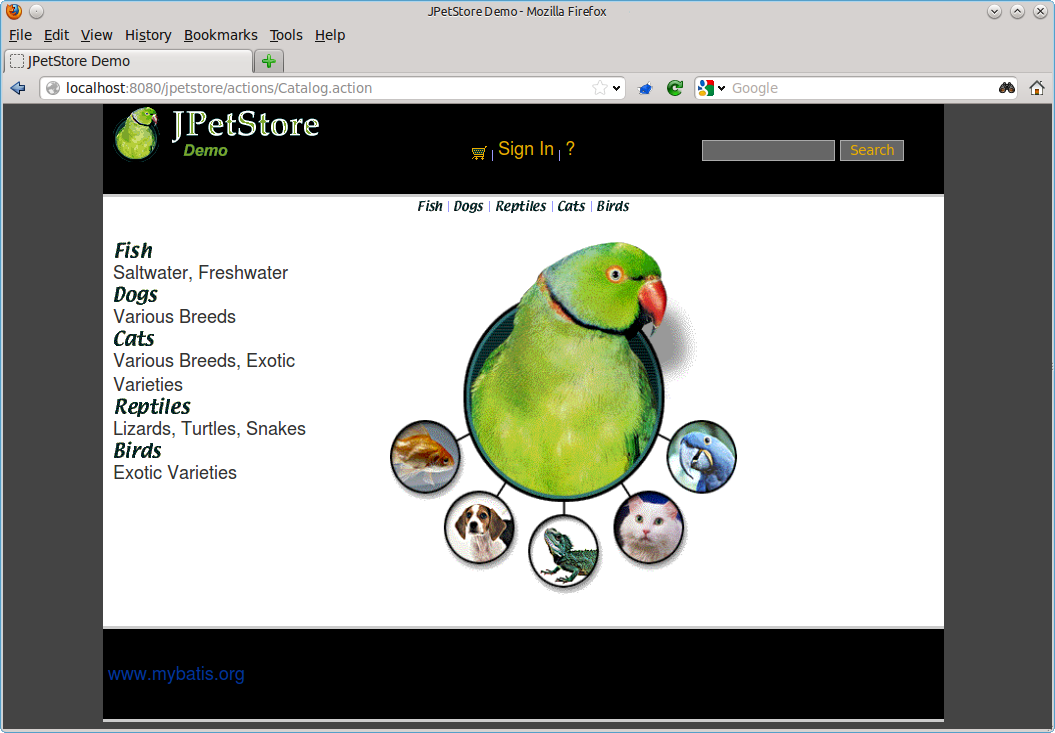
\includegraphics[width=0.45\textwidth]{images/jpetstore-example-FFscrsh}}
\hfill
\subfigure[\KiekerMonitoringPart{} control servlet]{\label{fig:controlServlet}%
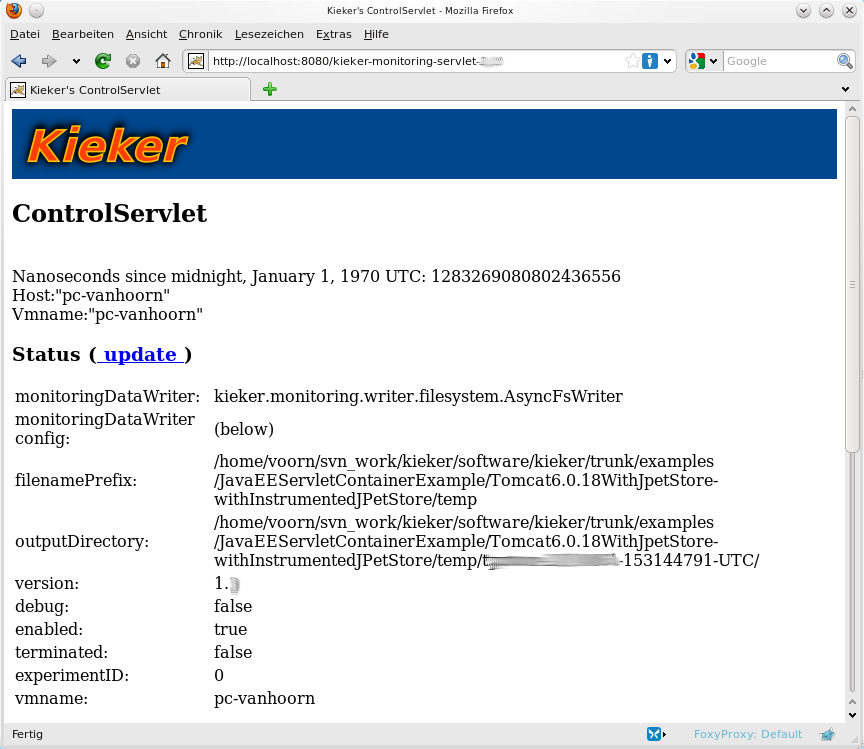
\includegraphics[width=0.45\textwidth]{images/kieker-servlet-FFscrsh-version-obfuscated}}
\hfill
\caption{}
\end{figure}

\newpage

\section{Rebuilding the JPetStore Application}\label{sec:Appendix:JPetStoreExample:rebuild}

\noindent In order to rebuild the JPetStore sources (located in \dir{JPetStore-5.0-instrumented/}), 
the following steps are required:

\

\begin{compactenum}
\item Copy the \file{\mainJar{}} from \Kieker{}'s
   binary distribution to the JPetStore's \dir{devlib/} directory. %
   It is required for the annotation-based instrumentation %
   (\texttt{@Ope\-rationExecutionMonitoringProbe}), as described in Chapter~\ref{chap:aspectJ}
\item Build the JPetStore with the \file{build.xml} by calling \texttt{ant} from %
    within \dir{build/} directory. 
\item You'll find the packaged JPetStore \file{.war}-file in \dir{build/wars/}.
\item Copy the file to the Tomcat's \dir{webapps/} directory.
\end{compactenum}

